% TODO: Falar que utilizamos o hit rate para ver se nossos modelos eram capazes de pelo menos prever quando que vai diminuir e quando que vai aumentar

% TODO: Melhorar os gráficos

% TODO?: Adicionar gráfico que mostra o tempo de predição

% TODO: Adicionar gráfico de como os modelos se comportam com o aumento do tamanho da janela

% TODO: Adicionar gráfico de como os modelos se comportam com o aumento da visão do passado

% TODO: Adicionar gráfico de como os modelos se comportam com o aumento e diminuição do intervalo de fluxo 

Este capítulo tem como objetivo apresentar uma discussão acerca dos resultados dos experimentos. Primeiramente, serão discutidos como os modelos reagem à variação dos principais parâmetros, tamanho de janela, passado visível e tamanho do intervalo do fluxo. Subsequentemente, será feita uma breve análise da melhora das predições dos modelos ao se utilizar dados normalizados. Após essa breve análise serão discutidos como os modelos reagem para a escolha dos valores de hiper-parâmetros. Por fim, serão discutidos os resultados das previsões de fluxo de cada modelo nos curtos prazos de 15, 30, 45 e 60 minutos.

\section{Resultados das escolhas de Parâmetros}

Após o tratamento dos dados, foram realizados diversos testes para definir os melhores parâmetros de cada modelo. Na lista abaixo podem ser vistos os parâmetro que foram levados em consideração nos estudos de caso deste trabalho.


\begin{enumerate}
	\item Tamanho da Janela: tamanho da janela utilizada para separar o conjunto de dados em treinamento e teste. O primeiro valor considerado foi 0.30. A partir deste valor inicial, o valor foi aumentado em 0.05 até atingir 0.85
	\item Passado Visível: Parâmetro que define qual a janela de tempo no passado que será visível no treinamento do modelo. O valor inicial considerado foi de 60 minutos. Os valores de 120, 180, 210. 240, 270, 300, 360 e 420 minutos também foram testados.
	\item Tamanho do intervalo do fluxo: Parâmetro que define o intervalo de tempo no qual será acumulado a quantidade de veículos para o cálculo do fluxo. O valor inicial de teste foi 60 minutos. Foram realizados testes para as variações de 150, 300 e 450 minutos também.
\end{enumerate}


\begin{figure}[H]
    \centering
    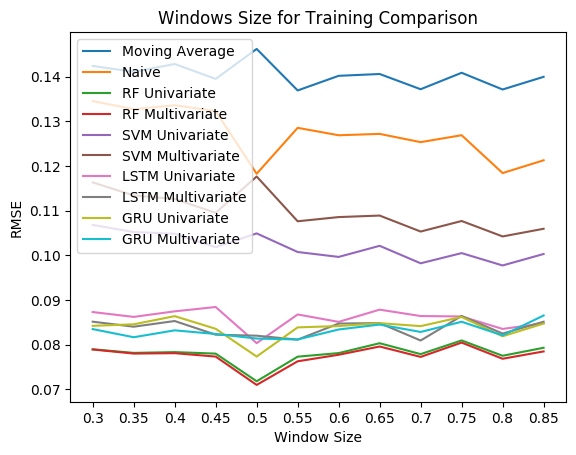
\includegraphics[scale=0.8]{monography/img/windows_size_for_training_comparison_rmse.png}
    \label{figure:rf}
    \caption[Resposta dos modelos à variação dos valores de tamanho de janela]{Resposta dos modelos à variação dos valores de tamanho de janela}
\end{figure} 


Como pode ser observado no gráfico acima, os modelos de aprendizagem de máquina, no geral, tiveram um melhor desempenho com uma janela de 0.5. Dentre eles, o melhor desempenho foi o do \acrshort{RF}

\begin{figure}[H]
    \centering
    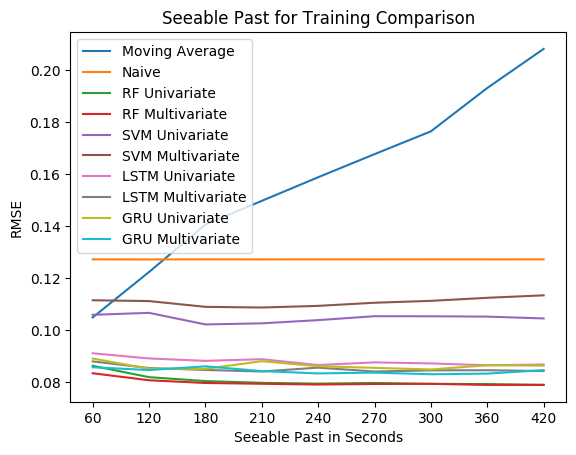
\includegraphics[scale=0.8]{monography/img/seeable_past_for_training_comparison_rmse.png}
    \label{figure:rf}
    \caption[Resposta dos modelos à variação dos valores de passado visível]{Resposta dos modelos à variação dos valores de passado visível}
\end{figure}

Quanto à resposta dos modelos em relação à variação do passado visível, é perceptível que a mudança do valor deste parâmetro não teve tanto impacto na predição dos modelos de aprendizagem de máquina e aprendizagem de máquina profunda. Porém, observando a média móvel, podemos perceber que a raíz do erro quadrado médio sobe quase que linearmente à medida que o passado visível aumenta.

\begin{figure}[H]
    \centering
    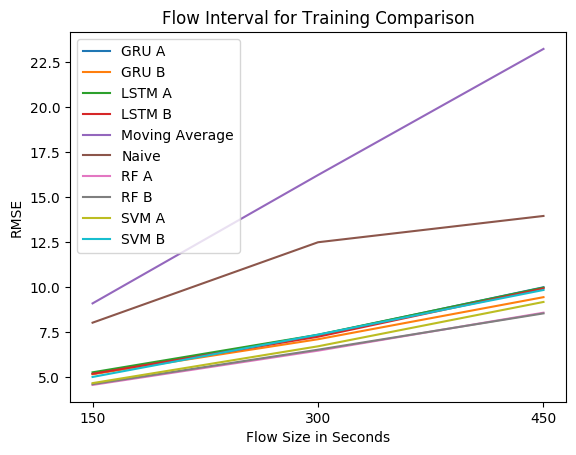
\includegraphics[scale=0.8]{monography/img/flow_interval_for_training_comparison_rmse.png}
    \label{figure:rf}
    \caption{Resposta dos modelos à variação dos valores de intervalo de fluxo \textit{\acrshort{}}\footnotemark}
\end{figure}


Por último, pode-se notar que o tamanho do intervalo do fluxo adotado impacta de maneira significativa a qualidade das predições dos modelos. Em todos os casos o erro quadrado médio das predições diminuiu com intervalos de fluxo maiores sendo utilizados durante o treinamento. Isso se dá pelo fato de que ao se aumentar o intervalo de fluxo, diminui-se a quantidade de ruídos presentes.


\section{Resultados das normalização dos Dados}

%TODO: COLOCAR REFERENCIA
Também é válido notar que os valores de entrada dos modelos estão normalizados. Para os modelos uni-variados, normalizamos o valor do fluxo utilizando a biblioteca \textit{Sklearn}, onde o menor valor é mapeado como 0 e o maior valor como 1. Segundo [Citar fonte que mostra que dados normalizados tendem a ter um melhor resultado], valores normalizados entre 0 e 1 tendem a ter um melhor resultado para algoritmos que utilizam funções de ativação sigmoidais, além de evitar que o modelo fique enviesado para os valores com maiores ordens de grandeza. Porém, como pode ser visto na tabela 1, no caso do \acrfull{LSTM}, o \acrfull{RMSE} ficou levemente menor para as predições utilizando valores normalizados em seu treinamento. Este aumento pouco significativo na melhora das predições pode ser justificado pelo fato dos valores dos intervalos do fluxo oriundo dos dados deste trabalho não serem tão grandes, sendo o menor valor 0 e o maior valor 60. Com um intervalo como esse, a normalização pode não ter tido um impacto tão significativo, pois 0 e 60 estão apenas a uma ordem de grandeza de diferença.

\begin{table}[H]
    \caption{Comparação das predições para os modelos univariados com e sem normalização para predições de 15 minutos}
    \label{table:RmseComparison}
    \begin{center}
    \begin{tabular}{ccccccc}
    \hline
    \multicolumn{1}{l}{\textbf{Modelo}} & \multicolumn{1}{l}{\textbf{RMSE-Norm.}} & \multicolumn{1}{l}{\textbf{RMSE-Não Norm.}}\\
    \hline
    SVM & 4.14 & 0.47  \\
    Mean & 6.20 & 0.71  \\
    Random Guess & 18.23 & 2.11\\
    GRU & 4.48 & 0.51  \\ 
    LSTM Mult & 4.99 &  0.57  \\ 
    LSTM Uni & 4.74 &  0.54  \\ 
    Random Forest & 4.17 & 0.48 \\
    \hline
    \end{tabular}
    \end{center}
\end{table}


O mesmo raciocínio pode ser utilizado para explicar a tabela 2, onde podemos observar que a normalização também não trouxe grandes benefícios aos modelos multivariados. Novamente, a ordem de grandeza entre os dados de entrada e entre os seus diferentes tipos (velocidade, fluxo, densidade) é bastante pequena, tornando a normalização pouco eficaz também nos casos dos modelos multivariados.

\begin{table}[H]
    \caption{Comparação das predições para os modelos multivariados com e sem normalização para predições de 15 minutos}
    \label{table:RmseComparison}
    \begin{center}
    \begin{tabular}{ccccccc}
    \hline
    \multicolumn{1}{l}{\textbf{Modelo}} & \multicolumn{1}{l}{\textbf{RMSE-Norm.}} & \multicolumn{1}{l}{\textbf{RMSE-Não Norm.}}\\
    \hline
    SVM & 4.14 & 0.47  \\
    Mean & 6.20 & 0.71  \\
    Random Guess & 18.23 & 2.11\\
    GRU & 4.48 & 0.51  \\ 
    LSTM Mult & 4.99 &  0.57  \\ 
    LSTM Uni & 4.74 &  0.54  \\ 
    Random Forest & 4.17 & 0.48 \\
    \hline
    \end{tabular}
    \end{center}
\end{table}

\section{Resultados das escolhas de Hiper-parâmetros}

O próximo passo foi escolher os melhores valores de hiper-parâmetros de cada modelo. Para os modelos de aprendizagem de máquina e aprendizagem profunda utilizou-se a biblioteca \textit{Hyperas} para descobrir os melhores valores dos seguintes hiper-parâmetros:

\begin{itemize}
	\item Quantidade de Neurônios da Rede: os valores testados foram 50 e 100.
	\item Tamanho do batch: os valores testados foram 16, 32 e 64.
	\item Função de ativação: foram testadas as funções sigmoid e relu.
	\item Número de épocas: os valores testados foram 15,20,25.
\end{itemize}

Abaixo podem ser vistos os valores resultantes dos testes para cada modelo:

\begin{table}[H]
    \caption{Melhores hiper-parâmetros para cada modelo de Aprendizagem de Máquina}
    \label{table:hiper-param-lstm}
    \begin{center}
    \begin{tabular}{ccccccc}
    \hline
    \multicolumn{1}{l}{\textbf{Modelo}} & \multicolumn{1}{l}{\textbf{Neurônios}} & \multicolumn{1}{l}{\textbf{Tam. Batch}} & \multicolumn{1}{l}{\textbf{Func. Ativação}} & \multicolumn{1}{l}{\textbf{Número de Épocas}}\\
    \hline
    LSTM Mult & 4.99 &  0.57 & 3.58  \\ 
    LSTM Uni & 4.74 &  0.54 & 3.37  \\
    GRU Mult & 4.99 &  0.57 & 3.58  \\ 
    GRU Uni & 4.74 &  0.54 & 3.37  \\
    \hline
    \end{tabular}
    \end{center}
\end{table}


\begin{table}[H]
    \caption{Melhores hiper-parâmetros para RF e SVM}
    \label{table:hiper-param}
    \begin{center}
    \begin{tabular}{ccccccc}
    \hline
    \multicolumn{1}{l}{\textbf{Modelo}} & \multicolumn{1}{l}{\textbf{Neurônios}} & \multicolumn{1}{l}{\textbf{Tam. Batch}} & \multicolumn{1}{l}{\textbf{Func. Ativação}} & \multicolumn{1}{l}{\textbf{Número de Épocas}}\\
    \hline
    SVM Mult & 4.99 &  0.57 & 3.58  \\ 
    SVM Uni & 4.74 &  0.54 & 3.37  \\
    RF Mult & 4.99 &  0.57 & 3.58  \\ 
    RF Uni & 4.74 &  0.54 & 3.37  \\
    \hline
    \end{tabular}
    \end{center}
\end{table}


%TODO: COLOCAR GRÁFICOS

Como pode ser visto nos gráficos/tabelas acima, todos os modelos tiveram uma melhora de performance ao serem utilizados os parâmetros resultantes dos testes.

\section{Teste de Predição para 15, 30, 45 e 60 minutos}

Por fim, após refinar todos os modelos e chegar às suas melhores versões, foram realizados os testes de predição para 15, 30, 45 e 60 minutos.

\begin{figure}[H]
    \centering
    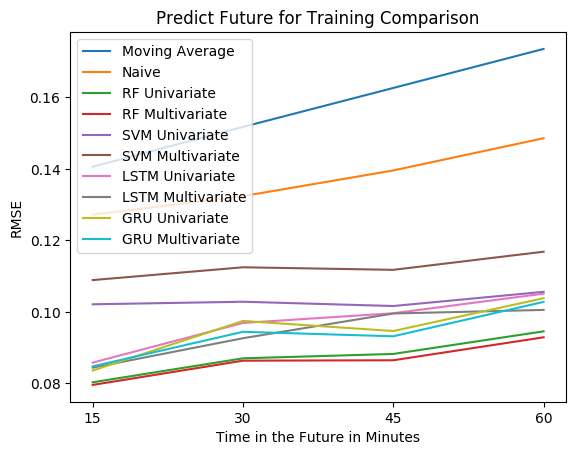
\includegraphics[scale=0.8]{monography/img/predict_future_for_training_comparison_rmse.png}
    \label{figure:rf}
    \caption{Comparação da predição dos modelos para diferentes valores de X minutos no futuro \textit{\acrshort{}}\footnotemark}
\end{figure}


Com todos os modelos nas suas melhores versões, com os valores mais adequados de parâmetros e hiper-parâmetros, realizamos um teste comparando todos os modelos com o mesmo conjunto de dados e para os seguintes valores de Janela: 


Como pode ser visto na tabela X,  todos  os  modelos  de aprendizagem  profunda  (LSTM  uni-variado  e  multi-variado,RNN  e  GRU)  tiveram  resultados  semelhantes,  mas  não  tão bons quanto os de aprendizagem supervisionada comum, como o random forest. Isso  pode  ter  acontecido  devido  ao  nosso  conjunto  de dados  e  seu  tamanho.  Redes  neurais  recorrentes  precisam de  um  grande  volume  de  dados  para  mapear  e  aprender  a sua  distribuição,  ao  contrário  de  modelos  de  aprendizagem supervisionada  tradicionais, que obtiveram melhores previsões com o nosso dataset.

Outro  ponto  interessante  a  se  notar ao observar a tabela y  é  o  tempo  de  treinamento de cada método. Os modelos de aprendizagem profunda tiveram um tempo de treinamento consideravelmente maior se comparado aos demais, o que é esperado, visto que possuem muito mais camadas de processamento. Já os  modelos  utilizados  como  base  de  comparação  tiveram um  tempo  de treinamento  extremamente  rápido,  pois  são métodos triviais  e  não  exigem  muito  processamento  e,  por consequência, também tiveram as piores previsões.


\begin{table}[H]
    \caption{Tabela Y com tempo de treinamento de cada modelo}
    \label{table:RmseComparison}
    \begin{center}
    \begin{tabular}{ccccccc}
    \hline
    \multicolumn{1}{l}{\textbf{Modelo}} & \multicolumn{1}{l}{\textbf{RMSE}} & \multicolumn{1}{l}{\textbf{NRMSE}} & \multicolumn{1}{l}{\textbf{MAE}} \\
    \hline
    SVM & 4.14 & 0.47 & 2.82  \\
    Mean & 6.20 & 0.71 & 4.55 \\
    Random Guess & 18.23 & 2.11 & 14.93\\
    RNN & 4.29 & 0.49 & 2.96 \\ 
    GRU & 4.48 & 0.51 & 3.11  \\ 
    LSTM Mult & 4.99 &  0.57 & 3.58  \\ 
    LSTM Uni & 4.74 &  0.54 & 3.37  \\ 
    Random Forest & 4.17 & 0.48 & 2.91 \\
    \hline
    \end{tabular}
    \end{center}
\end{table}